\documentclass[12pt,letterpaper]{article}


%\usepackage{amsthm}
\usepackage{multirow}
\usepackage{graphicx}
%\usepackage{epsfig}
%\usepackage{subfigure}
\usepackage{amsmath}
\usepackage{indentfirst}
\usepackage{amssymb}
\usepackage{cases}
\usepackage{ dsfont }
\usepackage[figuresright]{rotating}
\usepackage{float}
%\usepackage{subfigure}
\usepackage{caption}
 \usepackage{subcaption}
\usepackage[superscript,biblabel]{cite}

\DeclareMathOperator*{\argmax}{arg\,max}

\usepackage{setspace}
\onehalfspacing


\newtheorem{theorem}{Theorem}
\newtheorem{lemma}{Lemma}
\newtheorem{alg}{Algorithm}
\newtheorem{definition}{Definition}
%{\noindent{\bfseries Proof}}
\newcommand{\Proof}{\noindent{\bfseries Proof}}
\newcommand{\be}{\begin{equation}}
\newcommand{\ee}{\end{equation}}
\newtheorem{corollary}{Corollary}
\newtheorem{proposition}{Proposition}
\newtheorem{conjecture}{Conjecture}


\newcommand{\MyTabs}{ \hspace*{15.mm} \= ... \kill }


\usepackage[top=1in, left=1in, right=1in, bottom=1in]{geometry}

\newcommand{\tinyth}{\mbox{{\tiny{th}}}}
\newcommand{\tinyst}{\mbox{{\tiny{st}}}}

\usepackage{sectsty}

\sectionfont{\fontsize{12}{15}\selectfont}

\usepackage{abstract}
\renewcommand{\abstractname}{}    % clear the title
\renewcommand{\absnamepos}{empty} % originally center

\begin{document}
\renewcommand{\refname}{REFERENCES}

\title{XXX}

\author {xxx}%\Large 

\date{}

\maketitle

\begin{abstract}
\noindent\looseness-1
xxx
\end{abstract}

%\begin{keywords}
%Virtual Age, Remote Transmission, Finite Horizon\\
%\end{keywords}
%\centerline{\textsc{acronyms}}
%\begin{tabbing} \MyTabs
%PM\>preventive maintenance \\
%\end{tabbing}
%\centerline{\textsc{notation}}
%\begin{tabbing} \MyTabs
%$L$\> initial system lifetime \\
%\end{tabbing}


%\section*{Introduction}\label{sec:Intro}
%\baselineskip 20pt plus .3pt minus .1pt
\looseness - 1


\section*{A model of Continuous Time Markov Chain (CTMC) }\label{sec:Semi Markov Process (SMP)}
\looseness - 1
Consider a two state problem with states: $S=\{1,2\}$ . The changing rate between different states is either constant or duration dependent. The process is the CTMC in the first case and SMP in the second one.


We have two separate markov chains of this type. However, the probability of remaining in those states differs in these two markov chains. For instance, in the first chain this probability in states 1 and 2 is $80\%$ and $20\%$ and in the second chain is vice verse. The objective is to minimize the difference of this probability with the average $(50\%)$. 

A continuous-time stochastic process is a markov process which has a countable state space that can change its state at any point of time. Let $S_n$, be the $n^{th}$ transition time, $Y_n= S_n-S_{n-1}$ be the $n^{th}$ intertransition time (sojourn time) and $X_n$ be the state of system after $n^{th}$ transition (Kulkarni 2010). The integer-valued stochastic process $\{N(t); t\geq0 \}= sup\{n\geq0 : \Sigma_{i=0}^n X_i \leq t\}$ is a counting process generated by $\{Y_n, n\geq1\}$.

Therefore, the stochastic process $\{X_0, (X_n, Y_n), n\geq 1\}$ is called an CTMC if it satisfies 
\begin{equation}
P(X_{n+1}=j, Y_{n+1}\le y |X_n=i, Y_n, X_{n-1}, Y_{n-1},..., X_1, Y_1, X_0)
=P(X_1=j, Y_1\le s |X_0=i)
\end{equation}


We first model this problem as a single Markov chain with two states:

Consider the following CTMC with two states. If the system goes to state 1, it will stay there for an $exp(\lambda)$ amount of time and if it goes to state 2, it will remain there for an $exp(\mu)$ amount of time. Let $q_{ij}$ be the rate of leaving state $i$ and going to state $j$. 

\begin{figure}
  \centering
    
      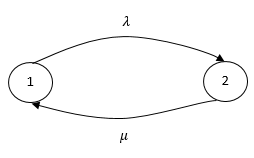
\includegraphics[width=0.5\textwidth]{CTMC}
  \caption{A model of CTMC with two states}
\end{figure}


Definition: The matrix Q=$[q_{ij}]$ is called the infinitesimal generator matrix (intensity matrix or transition rate matrix) for the CTMC. 

In this problem we have:

\[
Q=
\begin{bmatrix} 
-\lambda & \lambda \\
\mu & -\mu 
\end{bmatrix}
\]
Transient Analysis:

The transition probability of going from state $i$ to state $j$ at time $t$ is defined as following:
\begin{equation}
P_{ij}(t)=P(X(t)=j|X(0)=i)
\end{equation}

The matrix $P(t)$ is consist of $P_{ij}(t)$ as elements. Based on the following theorem, we can compute these transition probablities:

Theorem: (Forward and Backward Equations) $\forall t\geq 0,$ the matrix P(t) is differentiable and satisfies:

\begin{equation}
\frac{d}{dt}P(t)=P'(t)= Q.P(t) (Backward)
\end{equation}

\begin{equation}
\frac{d}{dt}P(t)=P'(t)= P(t).Q (Forward)
\end{equation}


For the problem which has two states we can have:

\[
P(t)=                                       
\begin{bmatrix} 
P_{11}(t) & P_{12}(t) \\
P_{21}(t) & P_{22}(t)
\end{bmatrix}\quad
Q=
\begin{bmatrix} 
-\lambda & \lambda \\
\mu & -\mu 
\end{bmatrix}
\]

By applying forward equations,


Forward equations:


\begin{equation}
\frac{d}{dt}P(t)=P'(t)= P(t).Q 
\end{equation}

\begin{equation}
P'_{11}(t)=-\lambda P_{11}(t)+\mu P_{12}(t)
\end{equation}

\begin{equation}
P'_{22}(t)=\lambda P_{21}(t)-\mu P_{22}(t)
\end{equation}

and using the fact that $\Sigma_k P_{ik}(t)=1$ for all $i$, we obtain,


\begin{equation}
P'_{11}(t)=\mu-(\lambda +\mu) P_{11}(t)
\end{equation}

\begin{equation}
P'_{22}(t)=\lambda-(\lambda +\mu) P_{22}(t)
\end{equation}


As always, we have initial conditions $P_{11}(0)=P_{22}(0)=1$,


Then we solve:


\begin{equation}
P_{11}(t)=\frac{\mu}{\lambda +\mu}+\frac{\lambda}{\lambda +\mu} e^{-(\lambda +\mu)t}
\end{equation}

\begin{equation}
P_{22}(t)=\frac{\lambda}{\lambda +\mu}+\frac{\mu}{\lambda +\mu} e^{-(\lambda +\mu)t}
\end{equation}


The ultimate goal is computing the total amount of time spent in each state. Since $P_{ii}(t)$ is the percentage of time spent in each state,therefore, we can obtain $T_i(t)$ as the following:

\begin{equation}
T_i(t)=P_{ii}(t)\times T
\end{equation}

where T is the time horizon (for example 8 hours).


Now, we can have the value of the total amount of time spent in each state of our problem for each arbitrary time horizon(for example 8 hours).

Consider the problem of having two states.  If the system goes to state 1, it will stay there for an $exp(3)$ amount of time and if it goes to state 2, it will remain there for an $exp(2)$ amount of time. We want to obtain the expected value of the total amount of time spent in each state for the time horizon of 8 hours. First we should compute the transition probabilities which we mentioned above:


$\lambda=3, \mu=2$


\begin{equation}
P_{11}(8)=\frac{2}{3 +2}+\frac{3}{3 +2} e^{-(3 +2)8}
\end{equation}

\begin{equation}
P_{22}(8)=\frac{3}{3 +2}+\frac{2}{3 +2} e^{-(3 +2)8}
\end{equation}


After computing the above equations, we have:
$P_{11}(8)=0.4$ and $P_{22}(8)=0.6$


Therefore, now we can compute the amount of time spent in these two states for the given time horizon (8 hours):

\begin{equation}
T_1(8)=P_{11}(t)\times T= 0.4 \times 8=3.2 hours
\end{equation}


\begin{equation}
T_2(8)=P_{22}(t)\times T= 0.6 \times 8=4.8 hours
\end{equation}

Now we want to compute the rates of $\lambda$ and $\mu$ in such a way that the system spend $80\%$ of the total amount of time horizon in state 1 and $20\%$ of the remaining in state 2. We can easily obtain these rates by using equations (10) and (11). Therefore,
we have $P_{11}(t)=0.8$ and $P_{22}(t)=0.2$,

\begin{equation}
0.8=\frac{\mu}{\lambda +\mu}+\frac{\lambda}{\lambda +\mu} e^{-(\lambda +\mu)8}
\end{equation}

\begin{equation}
0.2=\frac{\lambda}{\lambda +\mu}+\frac{\mu}{\lambda +\mu} e^{-(\lambda +\mu)8}
\end{equation}

So, from the above equations, we can estimate the relation of $\lambda$ and $\mu$:

\begin{equation}
4\lambda=\mu
\end{equation}








\section*{Acknowledgments}
The authors were partially supported by ...
%We also thank the Associate Editor and the anonymous referee for their insightful and constructive comments.



\bibliographystyle{plain}
*\bibliographystyle{unsrt}
*\bibliography{}


%\newpage
%\section{Appendix}\label{app:1}





\end{document}

